\documentclass[11pt]{article}

\usepackage[a4paper,margin=1in]{geometry}
\usepackage[T1]{fontenc}
\usepackage[utf8]{inputenc}
\usepackage{lmodern}
\usepackage{microtype}
\usepackage{amsmath,amssymb,amsthm,mathtools}
\usepackage{booktabs}
\usepackage{graphicx}
\usepackage{float}
\usepackage{placeins}
\usepackage{enumitem}
\usepackage[numbers,sort&compress]{natbib}
\usepackage{xcolor}
\usepackage{xurl}
\usepackage[colorlinks=true,linkcolor=blue!55!black,citecolor=blue!55!black,urlcolor=blue!55!black]{hyperref}
\usepackage[nameinlink,noabbrev]{cleveref}

\setlength{\parindent}{1.4em}
\setlength{\parskip}{0.15em}
\setlist{itemsep=0.25em,topsep=0.35em}

\newtheorem{theorem}{Theorem}[section]
\newtheorem{proposition}[theorem]{Proposition}
\newtheorem{lemma}[theorem]{Lemma}
\newtheorem{corollary}[theorem]{Corollary}
\theoremstyle{definition}
\newtheorem{definition}[theorem]{Definition}
\theoremstyle{remark}
\newtheorem{remark}[theorem]{Remark}

\newcommand{\R}{\mathbb R}
\newcommand{\C}{\mathbb C}
\newcommand{\uc}{u_{\mathrm c}}
\newcommand{\Id}{\mathrm I}
\newcommand{\cK}{\mathcal K}
\newcommand{\cA}{\mathcal A}
\newcommand{\cB}{\mathcal B}
\newcommand{\cC}{\mathcal C}
\newcommand{\cF}{\mathcal F}
\newcommand{\cG}{\mathcal G}
\newcommand{\cH}{\mathcal H}
\newcommand{\cM}{\mathcal M}
\newcommand{\cR}{\mathcal R}
\newcommand{\Ran}{\operatorname{Ran}}
\newcommand{\spec}{\operatorname{spec}}
\newcommand{\dist}{\operatorname{dist}}
\newcommand{\tr}{\operatorname{tr}}
\newcommand{\wind}{\operatorname{wind}}

\title{\textbf{Contour Feshbach Root Counting}\
\textbf{at a Quadratic Band-Merging Map:}\\[0.35em]
\large Blind Resonance Prediction, Holomorphic Shifted Krylov Reduction,\\
and a Narrow Isolation Corridor}
\author{Liang Wang\\
\small School of Artificial Intelligence and Automation,\\[-0.2em]
\small Huazhong University of Science and Technology, Wuhan 430074, P.R. China\\
\small \texttt{wangliang.f@gmail.com}}
\date{July 2026}

\begin{document}

\maketitle

\begin{abstract}
A packet--complement Feshbach closure can reproduce a physical eigenmode
when that eigenmode is already known, but this does not yet constitute a
spectral prediction.  We close that gap for finite noisy transfer matrices
at the first band-merging parameter of $f_u(x)=1-u x^2$.  For an oblique
packet pair $WV=\Id$, put $P=VW$, $Q=\Id-P$, and let $A$ be the
Perron/parity-extracted physical two-step operator.  On
$\C^m\oplus\Ran Q$, define
\[
 D=WAV,\qquad C=QAV,\qquad E=WAQ,\qquad
 B=QAQ\big|_{\Ran Q}.
\]
Whenever $z\notin\spec B$, the exact Feshbach matrix is
\[
 F(z)=z\Id-D-E(z\Id-B)^{-1}C.
\]
We prove the finite-dimensional determinant, compressed-resolvent, and
argument-principle identities
\[
 \det(z\Id-A)=\det(z\Id-B)\det F(z),\qquad
 W(z\Id-A)^{-1}V=F(z)^{-1},
\]
\[
 \wind_\Gamma\det F=N_\Gamma(A)-N_\Gamma(B).
\]

To evaluate $F$ on an entire contour without destroying analyticity in
$z$, every column of $C$ is reduced by a shift-invariant Arnoldi--FOM
space.  The resulting rational matrix $F_J(z)$ is the exact Schur
complement of an explicit augmented matrix $M_J$ and therefore satisfies
\[
 \det(z\Id-M_J)
 =\prod_{i=1}^m\det(z\Id-H_{i,J})\det F_J(z).
\]
We also give an exact Arnoldi residual formula, a floating-point recurrence
defect bound, and a conditional matrix-Rouch\'e criterion transferring the
projected count to the exact $F$.  The missing ingredient for a validated
transfer is an upper bound on the external resolvent; sampled depth
comparisons are not substituted for that theorem.

The numerical protocol is target-blind.  It uses only the two real
peripheral modes and the rightmost lower-half-plane eigenvalue of $D$ to
choose concentric discovery contours.  Nonreal full-matrix eigenvalues are
computed only after the Feshbach root is frozen.  Across seven noise scales
$10^{-2}\ge\sigma\ge10^{-4}$, dimensions $2048\le n\le204800$, packet
ranks $4\le m\le9$, and Arnoldi depths $36\le J\le62$, every selected
contour has winding one, no projected pole, one augmented zero, and one
captured outer full-matrix eigenvalue.  Direct packet errors lie between
$4.71\times10^{-2}$ and $2.48\times10^{-1}$; contour-Feshbach prediction
errors lie between $1.36\times10^{-15}$ and $3.47\times10^{-14}$.  The
largest computable Arnoldi residual bound is $1.93\times10^{-11}$, and the
largest sampled $J-8$ to $J$ Rouch\'e ratio is $4.59\times10^{-6}$.  The
pole-free one-root corridors remain open but narrow to widths of order
$10^{-2}$.  Six packet-window variants preserve winding one, with maximum
prediction error $6.01\times10^{-13}$.  These are reproducible
floating-point results for finite discretizations, not a validated
continuum or small-noise theorem.
\end{abstract}

\noindent\textbf{Keywords:} Feshbach map; argument principle; Arnoldi
method; nonlinear eigenvalue problem; oblique projection; Gaussian transfer
operator; nonnormal spectrum; quadratic map.

\medskip
\noindent\textbf{MSC 2020:} 37E05; 47A10; 47A55; 47B65; 65F15; 65P30.

\section{Introduction}
\label{sec:introduction}

Finite-rank reductions of nonnormal transfer operators face a basic
distinction.  A reduced model can \emph{explain} a known eigenpair, or it can
\emph{predict} an eigenvalue without using that eigenpair.  The first task is
an algebraic closure test; the second requires a spectral parameter, a
contour on which the discarded complement is solved, and a stable root
count.  This paper performs the second task for the physical small-noise
operator at a quadratic band-merging map.

The preceding construction began with a parity-extracted bulk scattering
model and an exact endpoint pole \citep{WangBulkScattering2026}.  A
time-ordered boundary word and Gaussian packet propagation then identified
the relevant cycle and its physical realization
\citep{WangTimeOrdered2026,WangGaussianReturn2026}.  Subsequent work tested
the branch and complement structure.  One-branch closure misses an
order-one sibling contribution; an unconstrained time lift produces
Floquet copies rather than new physical attenuation
\citep{WangComplement2026}.  Two critical branches yield a nearly rank-one
bright channel, while peripheral biorthogonalization gives a valid oblique
packet projector and exposes branch-history collapse
\citep{WangSectorBranch2026,WangBiorthogonal2026}.  A scalar local dark
channel has the wrong sign or insufficient self-energy, ruling out that
shortcut \citep{WangDarkSchur2026}.

The full packet complement was therefore retained in
\citet{WangPhysicalFeshbach2026}.  That work corrected the spectral target:
if $K_{\mathrm b,\sigma}r_\sigma=\mu_\sigma r_\sigma$, the exact two-step
eigenvalue is the complex number $\nu_\sigma=\mu_\sigma^2$, not the positive
radius $|\mu_\sigma|^2$.  It proved the exact packet and external block
equations and found that the packet component of the right eigenvector
shrinks while the external resolvent becomes increasingly ill-conditioned.
The compressed pole nevertheless stays visible because left weight and
resolvent amplification compensate the small right projection.  Crucially,
that audit inserted the already known physical eigenpair into the block
equations.  It validated the mechanism but did not independently locate a
root.

The present paper makes four advances.

\begin{enumerate}[label=\textbf{C\arabic*.},leftmargin=2.8em]
 \item \textbf{Exact contour count.}  The oblique Feshbach determinant is
 related to the full and external characteristic polynomials.  Its winding
 equals the number of full eigenvalues minus external eigenvalues inside a
 contour.
 \item \textbf{Holomorphic shifted reduction.}  Independent Arnoldi spaces
 for the columns of $QAV$ produce one rational matrix $F_J(z)$ valid for all
 shifts.  The dependence on $z$ remains holomorphic away from projected
 poles, which is essential for the argument principle.
 \item \textbf{Projected count and conditional transfer.}  An explicit
 augmented matrix makes the projected zero-minus-pole count exact.  An
 Arnoldi residual identity and matrix-Rouch\'e condition isolate precisely
 what is still required to transfer that count rigorously to the original
 external block.
 \item \textbf{Blind finite-matrix prediction.}  The nonreal reference
 eigensystem is withheld until after the contour and root are frozen.  Seven
 scales, depth variation, node refinement, and packet-window variation test
 the resulting prediction.
\end{enumerate}

The evidence hierarchy is important.  The Schur identities, augmented
determinant identity, and conditional error criterion are exact
finite-dimensional statements.  The winding and root counts for $F_J$ are
floating-point evaluations of an explicit rational matrix, cross-checked by
ordinary eigenvalue counts of $M_J$.  Agreement with the later full-matrix
reference is numerical evidence for the physical finite discretization.
No interval enclosure of the contour, no validated upper external-resolvent
bound, and no continuum or $\sigma\downarrow0$ theorem is claimed.

\section{Physical operator, packet pair, and blind protocol}
\label{sec:physical}

\subsection{Perron/parity-extracted two-step operator}

Let
\[
 f_u(x)=1-u x^2
\]
at the first algebraic band-merging parameter $u=\uc$.  The discretization
used below is the folded Gaussian Markov matrix $K_\sigma^{(n)}$ on positive
midpoints, with the dimension rule $n\sigma=20.48$.  Its construction and
normalization are inherited unchanged from the earlier sparse-operator
audit \citep{WangBulkScattering2026,WangPhysicalFeshbach2026}.

Let $R_\perp,L_\perp\in\R^{n\times2}$ contain the right and left Perron and
parity modes, normalized by
\[
 L_\perp^{\mathsf T}R_\perp=\Id_2,
\qquad
 \Lambda_\perp=\operatorname{diag}(\lambda_{\rm P},\lambda_{\rm par}).
\]
The one-step bulk operator and the physical two-step operator are
\begin{equation}
 K_{\mathrm b,\sigma}
 =K_\sigma^{(n)}-R_\perp\Lambda_\perp L_\perp^{\mathsf T},
 \qquad
 A_\sigma=K_{\mathrm b,\sigma}^2.
 \label{eq:bulk-two-step}
\end{equation}
Every contour calculation in this paper concerns the complex spectrum of
$A_\sigma$.  The positive return radius used in earlier cycle diagnostics
is not substituted for this complex target.

\subsection{Canonical packet and complement}

The packet trial matrix $V\in\R^{n\times m}$ is assembled from propagated
critical-branch histories.  Regular slices retain their normalized bright
sum and the final critical slice retains both disjoint branch labels.  The
canonical Petrov analysis $W\in\R^{m\times n}$ removes the two peripheral
modes and obeys
\begin{equation}
 WV=\Id_m.
 \label{eq:biorthogonal-pair}
\end{equation}
Thus
\[
 P=VW,
 \qquad Q=\Id-P
\]
are complementary, generally oblique projectors.  We use the direct packet
matrix
\begin{equation}
 D=W A_\sigma V
 \label{eq:direct-matrix}
\end{equation}
only as a target-free center generator.  Among its eigenvalues in the lower
half-plane, define
\begin{equation}
 z_{\rm d}
 =\underset{\lambda\in\spec D,\ \Im\lambda<0}{\operatorname{argmax}}
 \bigl(\Re\lambda,|\lambda|\bigr),
 \label{eq:direct-center-rule}
\end{equation}
where the second entry breaks ties.  No nonreal eigenvalue of
$K_\sigma^{(n)}$ appears in this rule.

\subsection{What ``blind'' means}
\label{sec:blind-definition}

The implementation separates construction and reference stages.

\begin{enumerate}
 \item A construction eigensolve requests eight largest-modulus left and
 right modes.  Only the two real Perron/parity modes are selected; all
 nonreal values and vectors are discarded from the returned object.
 \item The packet, $D$, the complement Krylov model, the discovery contour,
 the winding, and the nonlinear root are computed and frozen.
 \item A separate reference eigensolve then requests 24 outer left and right
 modes.  The unique captured two-step eigenvalue inside the frozen contour
 is reported as the blind reference.
\end{enumerate}

The construction eigensolver may internally traverse nonreal Krylov
directions, as any iterative eigensolver can.  Blindness here is an
information-flow statement: no nonreal Ritz value or vector is read, stored
in the construction object, used to select $z_{\rm d}$, or used to place the
contour.  The separate reference call occurs after the prediction.

\section{Exact oblique Feshbach algebra on a contour}
\label{sec:exact-feshbach}

Suppress the scale index and write $A=A_\sigma$.  On the complementary
decomposition $\C^n=\Ran P\oplus\Ran Q$, define
\begin{equation}
 D=WAV,\qquad C=QAV,\qquad E=WAQ,
 \qquad B=QAQ\big|_{\Ran Q}.
 \label{eq:block-definitions}
\end{equation}
Here $C:\C^m\to\Ran Q$, $E:\Ran Q\to\C^m$, and
$B:\Ran Q\to\Ran Q$.

\begin{theorem}[Oblique Feshbach factorization]
\label{thm:exact-feshbach}
For $z\notin\spec B$, set
\begin{equation}
 F(z)=z\Id_m-D-E(z\Id_{\Ran Q}-B)^{-1}C.
 \label{eq:exact-feshbach}
\end{equation}
Then
\begin{align}
 \det(z\Id_n-A)
 &=\det(z\Id_{\Ran Q}-B)\det F(z),
 \label{eq:exact-det-factorization}\\
 W(z\Id_n-A)^{-1}V&=F(z)^{-1}
 \label{eq:compressed-resolvent}
\end{align}
whenever the displayed inverses exist.
\end{theorem}

\begin{proof}
The map
\[
 S:\C^m\oplus\Ran Q\longrightarrow\C^n,
 \qquad S(\alpha,q)=V\alpha+q
\]
is an isomorphism with inverse $S^{-1}x=(Wx,Qx)$.  In these coordinates,
\[
 S^{-1}AS=
 \begin{pmatrix}
  D&E\\ C&B
 \end{pmatrix}.
\]
Taking the Schur complement of $z\Id-B$ proves
\cref{eq:exact-det-factorization}.  Block inversion gives the upper-left
block $F(z)^{-1}$, which is exactly
$W(z\Id-A)^{-1}V$.
\end{proof}

Let $\Omega$ be the interior of a positively oriented simple contour
$\Gamma$, and let $N_\Gamma(T)$ denote the algebraic number of eigenvalues
of $T$ in $\Omega$.

\begin{theorem}[Feshbach argument principle]
\label{thm:argument-principle}
Assume $\Gamma$ meets neither $\spec A$ nor $\spec B$.  Then
\begin{equation}
 \wind_\Gamma\det F
 =\frac{1}{2\pi i}\int_\Gamma
   \tr\!\left(F(z)^{-1}F'(z)\right)\,dz
 =N_\Gamma(A)-N_\Gamma(B).
 \label{eq:feshbach-count}
\end{equation}
In particular, if $N_\Gamma(B)=0$ and the winding is one, $\Gamma$ contains
exactly one eigenvalue of $A$, counted algebraically.
\end{theorem}

\begin{proof}
Apply the scalar argument principle to
\cref{eq:exact-det-factorization}.  Away from zeros and poles, Jacobi's
formula gives
\[
 \frac{(\det F)'}{\det F}=\tr(F^{-1}F'),
\]
as required \citep{Ahlfors1979,HornJohnson2013}.
\end{proof}

\begin{remark}[Meromorphic, not automatically analytic]
\label{rem:meromorphic}
The winding of $\det F$ is generally a zero-minus-pole count.  Calling it a
full eigenvalue count requires excluding external eigenvalues from the
interior, not merely solving the external equation at points on the
boundary.  This distinction motivates the projected pole audit below.
\end{remark}

\section{A holomorphic shifted Arnoldi Feshbach model}
\label{sec:arnoldi}

Directly solving $(z\Id-B)X=C$ for every contour node and every packet
column is expensive.  More importantly, an independently restarted
least-squares solve at each $z$ need not define one holomorphic matrix-valued
function of $z$.  The argument principle applies to a function, not to an
unrelated collection of pointwise approximations.  We therefore use the
shift invariance of polynomial Krylov spaces \citep{Saad1980,Saad2003}.

\subsection{Column-wise Arnoldi--FOM reduction}

Write $C=[c_1,\ldots,c_m]$.  For each column, construct a Euclidean
orthonormal Arnoldi basis
\[
 U_{i,J}=[u_{i,1},\ldots,u_{i,J}],
 \qquad c_i=\beta_i u_{i,1},
\]
with relation
\begin{equation}
 B U_{i,J}
 =U_{i,J}H_{i,J}
  +h_{i,J+1,J}u_{i,J+1}e_J^*.
 \label{eq:arnoldi-relation}
\end{equation}
The packet observation of this basis is
\[
 G_{i,J}=E U_{i,J}\in\C^{m\times J}.
\]
For every shift away from $\spec H_{i,J}$, define
\begin{equation}
 y_{i,J}(z)=(z\Id_J-H_{i,J})^{-1}\beta_i e_1,
 \qquad
 x_{i,J}(z)=U_{i,J}y_{i,J}(z).
 \label{eq:fom-solution}
\end{equation}
The projected self-energy and Feshbach matrix are
\begin{align}
 \Sigma_J(z)
 &=\bigl[G_{1,J}y_{1,J}(z),\ldots,G_{m,J}y_{m,J}(z)\bigr],
 \label{eq:projected-self-energy}\\
 F_J(z)&=z\Id_m-D-\Sigma_J(z).
 \label{eq:projected-feshbach}
\end{align}
Sparse applications of $B$ to the $m$ current Arnoldi vectors are batched,
but each column is orthogonalized only against its own basis.  This avoids
the quadratic cross-column orthogonalization cost of one large block basis.

\subsection{Exact augmented realization}

Let
\[
 \cH_J=\operatorname{diag}(H_{1,J},\ldots,H_{m,J}),
 \qquad
 \cG_J=[G_{1,J}\ \cdots\ G_{m,J}],
\]
and let $\cC_J\in\C^{mJ\times m}$ have $i$th block column
$\beta_i e_1$.  Define
\begin{equation}
 M_J=
 \begin{pmatrix}
  D&\cG_J\\
  \cC_J&\cH_J
 \end{pmatrix}.
 \label{eq:augmented-matrix}
\end{equation}

\begin{theorem}[Projected determinant identity]
\label{thm:projected-determinant}
For $z\notin\bigcup_i\spec H_{i,J}$,
\begin{equation}
 \det(z\Id_{m+mJ}-M_J)
 =\left[\prod_{i=1}^m\det(z\Id_J-H_{i,J})\right]\det F_J(z).
 \label{eq:projected-det-identity}
\end{equation}
Consequently,
\begin{equation}
 \wind_\Gamma\det F_J
 =N_\Gamma(M_J)-\sum_{i=1}^m N_\Gamma(H_{i,J})
 \label{eq:projected-count}
\end{equation}
for every contour avoiding the projected zeros and poles.
\end{theorem}

\begin{proof}
Take the Schur complement of $z\Id_{mJ}-\cH_J$ in
$z\Id-M_J$.  Its upper-left block is exactly $F_J(z)$.  The determinant
factorization and argument principle then give the two claims.
\end{proof}

This theorem gives two independent finite computations of the projected
count: phase winding of the small $m\times m$ determinant and ordinary
eigenvalue counts of $M_J$ and the $H_{i,J}$.  It also explains why the
column-wise realization produces repeated projected pole--zero clusters:
each right-hand side carries its own approximation of the external block.
Those clusters are numerical realization events, not automatically new
physical resonances.

\subsection{Derivative, moments, and Newton refinement}

Differentiating \cref{eq:projected-feshbach} gives the $i$th column of
$F_J'(z)$ as
\begin{equation}
 F_J'(z)e_i
 =e_i+G_{i,J}(z\Id_J-H_{i,J})^{-2}\beta_i e_1.
 \label{eq:feshbach-derivative}
\end{equation}
Thus the projected count and first moment are
\begin{align}
 n_J&=\frac{1}{2\pi i}\int_\Gamma
 \tr(F_J^{-1}F_J')\,dz,
 \label{eq:cauchy-count}\\
 s_J&=\frac{1}{2\pi i}\int_\Gamma
 z\,\tr(F_J^{-1}F_J')\,dz.
 \label{eq:cauchy-moment}
\end{align}
If the contour contains one zero and no pole, $s_J/n_J$ is its Cauchy
centroid.  A simple zero is refined by the log-determinant Newton step
\begin{equation}
 z_{k+1}=z_k-
 \left[\tr\!\left(F_J(z_k)^{-1}F_J'(z_k)\right)\right]^{-1},
 \label{eq:newton}
\end{equation}
as in contour methods for nonlinear eigenvalue problems
\citep{Beyn2012}.

\subsection{Residuals and the exact missing estimate}

In exact arithmetic, \cref{eq:arnoldi-relation} implies
\begin{equation}
 \frac{\|c_i-(z\Id-B)x_{i,J}(z)\|}{\|c_i\|}
 =\frac{|h_{i,J+1,J}e_J^*y_{i,J}(z)|}{\beta_i}.
 \label{eq:ideal-residual}
\end{equation}
At deep convergence this expression can fall below the floating-point
recurrence floor.  The implementation therefore records every actual
Arnoldi relation defect $d_{i,k}$.  If $y=(y_1,\ldots,y_J)^\mathsf T$, it
reports the computable bound
\begin{equation}
 \|c_i-(z\Id-B)x_{i,J}\|
 \le |h_{i,J+1,J}y_J|
    +\sum_{k=1}^J |y_k|\,\|d_{i,k}\|.
 \label{eq:floating-residual-bound}
\end{equation}
This prevents a formal $10^{-40}$ Krylov residual from being presented as
physical accuracy when the recurrence itself is accurate only near machine
precision.

Let $X_J=[x_{1,J},\ldots,x_{m,J}]$ and
\[
 R_J(z)=C-(z\Id-B)X_J(z).
\]

\begin{theorem}[Conditional transfer to the exact Feshbach count]
\label{thm:conditional-rouche}
Suppose $\Gamma$ and its interior avoid $\spec B$ and the poles of $F_J$.
Then
\begin{equation}
 F(z)-F_J(z)=-E(z\Id-B)^{-1}R_J(z).
 \label{eq:feshbach-error-identity}
\end{equation}
If
\begin{equation}
 \sup_{z\in\Gamma}
 \left\|F_J(z)^{-1}E(z\Id-B)^{-1}R_J(z)\right\|_2<1,
 \label{eq:exact-rouche-condition}
\end{equation}
then $F$ and $F_J$ have the same number of zeros inside $\Gamma$, counted
algebraically.
\end{theorem}

\begin{proof}
The residual identity gives
$(z\Id-B)^{-1}C-X_J=(z\Id-B)^{-1}R_J$ and hence
\cref{eq:feshbach-error-identity}.  The matrix-valued Rouch\'e theorem
applied to $F_J+(F-F_J)$ proves the count equality
\citep{GohbergSigal1971}.
\end{proof}

A sufficient scalar bound is
\begin{equation}
 \sup_\Gamma\|F_J^{-1}\|\,\|E\|\,
 \sup_\Gamma\|(z\Id-B)^{-1}\|\,
 \sup_\Gamma\|R_J\|<1.
 \label{eq:scalar-rouche-bound}
\end{equation}
The residual is computed, but no validated upper bound for the middle
external resolvent is available.  The experiment also reports
\begin{equation}
 \widehat\eta_{J-8,J}
 =\max_{z_\ell\in\Gamma}
 \left\|F_{J-8}(z_\ell)^{-1}
       \bigl(F_J(z_\ell)-F_{J-8}(z_\ell)\bigr)\right\|_2.
 \label{eq:sampled-rouche}
\end{equation}
This is a useful sampled depth-stability diagnostic.  It is not the
supremum in \cref{eq:exact-rouche-condition}, does not contain the exact
external resolvent, and is not advertised as a proof.

\section{Numerical design}
\label{sec:numerics}

\subsection{Seven scales and Krylov dimensions}

The baseline uses the canonical packet half-width of six local standard
deviations.  The sparse dimensions, component periods, packet ranks, and
Arnoldi depths are listed in \cref{tab:settings}.

\begin{table}[H]
\centering
\caption{Physical discretizations and column-wise Arnoldi depths.}
\label{tab:settings}
\begin{tabular}{rrrrr}
\toprule
$\sigma$ & $n$ & component period $k$ & packet rank $m$ & depth $J$\\
\midrule
$10^{-2}$        & $2{,}048$   & 3 & 4 & 36\\
$4\times10^{-3}$ & $5{,}120$   & 4 & 5 & 42\\
$2\times10^{-3}$ & $10{,}240$  & 5 & 6 & 46\\
$10^{-3}$        & $20{,}480$  & 6 & 7 & 50\\
$5\times10^{-4}$ & $40{,}960$  & 6 & 7 & 54\\
$2\times10^{-4}$ & $102{,}400$ & 7 & 8 & 58\\
$10^{-4}$        & $204{,}800$ & 8 & 9 & 62\\
\bottomrule
\end{tabular}
\end{table}

Each Arnoldi step applies $B$ to all $m$ current vectors in one sparse
matrix--matrix operation.  Two reorthogonalization passes are used.  The
maximum observed loss of orthogonality is below $3.10\times10^{-14}$.

\subsection{Discovery, isolation, and reference}
\label{sec:discovery-protocol}

For each scale the protocol is as follows.

\begin{enumerate}
 \item Compute $z_{\rm d}$ from \cref{eq:direct-center-rule}.
 \item Scan the 45 target-free circles
 \[
  \Gamma_\rho:\quad z=z_{\rm d}+\rho|z_{\rm d}|e^{i\theta},
  \qquad \rho=0.04,0.05,\ldots,0.48,
 \]
 using 128 nodes.  Retain circles with determinant winding one, projected
 pole count zero, and maximum phase increment below $0.85\pi$.
 \item Use the best-conditioned retained circle to obtain a Cauchy centroid
 and Newton root $z_J$.
 \item Compute the spectra of $M_J$ and the $H_{i,J}$.  Along the radial
 family centered at $z_{\rm d}$, let $r_*$ be the target-root radius and
 $r_{\rm next}$ the next projected zero or pole radius.  Place the final
 contour at
 \begin{equation}
  r_\Gamma=\frac{r_*+r_{\rm next}}{2}.
  \label{eq:mid-corridor}
 \end{equation}
 This maximizes radial clearance inside that one-root corridor.
 \item Recompute winding, Cauchy moments, residuals, and Newton refinement
 using 512 nodes.  Only then run the separate 24-mode reference eigensolve.
\end{enumerate}

The contour placement uses projected zeros and poles, which are part of the
constructed rational model; it never uses the withheld full-matrix target.
Every next event in the seven-scale baseline is a nearly coincident
projected pole--zero cluster.  We use the cluster as a conservative contour
barrier and do not interpret it as a physical resonance.

\subsection{Cross-checks}

Five checks are recorded.

\begin{enumerate}
 \item The phase winding of $\det F_J$ is compared with the augmented count
 $N_\Gamma(M_J)-\sum_iN_\Gamma(H_{i,J})$.
 \item Arnoldi depths $J-16$, $J-8$, and $J$ are compared on the same final
 contour.
 \item Contour node counts $64,96,128,192,256,384,512$ test phase and Cauchy
 quadrature stability.
 \item The 24 captured outer one-step eigenvalues are squared only after the
 prediction.  At every scale exactly one lies in the frozen contour.  The
 contour's radial floor exceeds the smallest captured two-step modulus, so
 the outer-spectrum comparison extends well below the contour, although it
 remains an ARPACK computation rather than an interval proof.
 \item Packet half-widths $5,6,7$ are tested at $\sigma=10^{-3}$ and
 $10^{-4}$.
\end{enumerate}

All calculations use NumPy and SciPy; figures use Matplotlib
\citep{HarrisEtAl2020,VirtanenEtAl2020,Hunter2007}.  Source, tests, CSV data,
small serialized rational models, and figures are archived with the paper
\citep{WangContourFeshbachCode2026}.

\section{Seven-scale root-count results}
\label{sec:results}

\subsection{The complement changes approximation into prediction}

The central result is summarized in \cref{tab:main-results}.  All seven
selected windings equal one.  All selected projected pole counts are zero,
all augmented counts are one, and exactly one captured outer full-matrix
eigenvalue lies in each frozen contour.  Twelve-step factorization spot
checks have maximum relative residual $1.59\times10^{-14}$, and the closest
maximum-depth augmented eigenvalue differs from the Newton root by at most
$7.94\times10^{-15}$.

\begin{table}[H]
\centering
\caption{Blind baseline predictions.  $e_D=|z_{\rm d}-z_{\rm ref}|$,
$e_F=|z_J-z_{\rm ref}|$, $r_J$ is the maximum floating Arnoldi residual
bound on the final contour, $\widehat\eta$ is
\cref{eq:sampled-rouche}, and $w$ is the absolute isolation-corridor width.}
\label{tab:main-results}
\resizebox{\textwidth}{!}{%
\begin{tabular}{rrrrrrr}
\toprule
$\sigma$ & $e_D$ & $e_F$ & $r_J$ & $\widehat\eta_{J-8,J}$ & $w$ & winding/poles/zeros\\
\midrule
$10^{-2}$        & $2.481\times10^{-1}$ & $2.57\times10^{-15}$ & $2.03\times10^{-15}$ & $7.40\times10^{-15}$ & $2.884\times10^{-2}$ & $1/0/1$\\
$4\times10^{-3}$ & $1.362\times10^{-1}$ & $1.36\times10^{-15}$ & $3.72\times10^{-15}$ & $1.72\times10^{-14}$ & $2.871\times10^{-2}$ & $1/0/1$\\
$2\times10^{-3}$ & $1.058\times10^{-1}$ & $1.79\times10^{-15}$ & $9.18\times10^{-15}$ & $5.52\times10^{-14}$ & $2.156\times10^{-2}$ & $1/0/1$\\
$10^{-3}$        & $9.005\times10^{-2}$ & $3.35\times10^{-15}$ & $2.81\times10^{-14}$ & $1.09\times10^{-13}$ & $1.200\times10^{-2}$ & $1/0/1$\\
$5\times10^{-4}$ & $5.096\times10^{-2}$ & $2.53\times10^{-15}$ & $1.80\times10^{-14}$ & $1.97\times10^{-8}$  & $2.167\times10^{-2}$ & $1/0/1$\\
$2\times10^{-4}$ & $4.710\times10^{-2}$ & $1.59\times10^{-14}$ & $1.40\times10^{-12}$ & $2.39\times10^{-6}$  & $1.662\times10^{-2}$ & $1/0/1$\\
$10^{-4}$        & $5.213\times10^{-2}$ & $3.47\times10^{-14}$ & $1.93\times10^{-11}$ & $4.59\times10^{-6}$  & $1.005\times10^{-2}$ & $1/0/1$\\
\bottomrule
\end{tabular}}
\end{table}

The direct packet matrix is not already the answer: its error remains
between $0.0471$ and $0.248$.  The full complement self-energy moves the
root to the later reference at floating-point accuracy.  The improvement
factor is at least $1.50\times10^{12}$ on the computed range.  This does not
mean twelve digits have been proved for an infinite-dimensional operator;
it means the converged rational Feshbach model reproduces the selected
finite sparse-matrix eigenvalue to the stated floating-point error.

\begin{figure}[H]
\centering
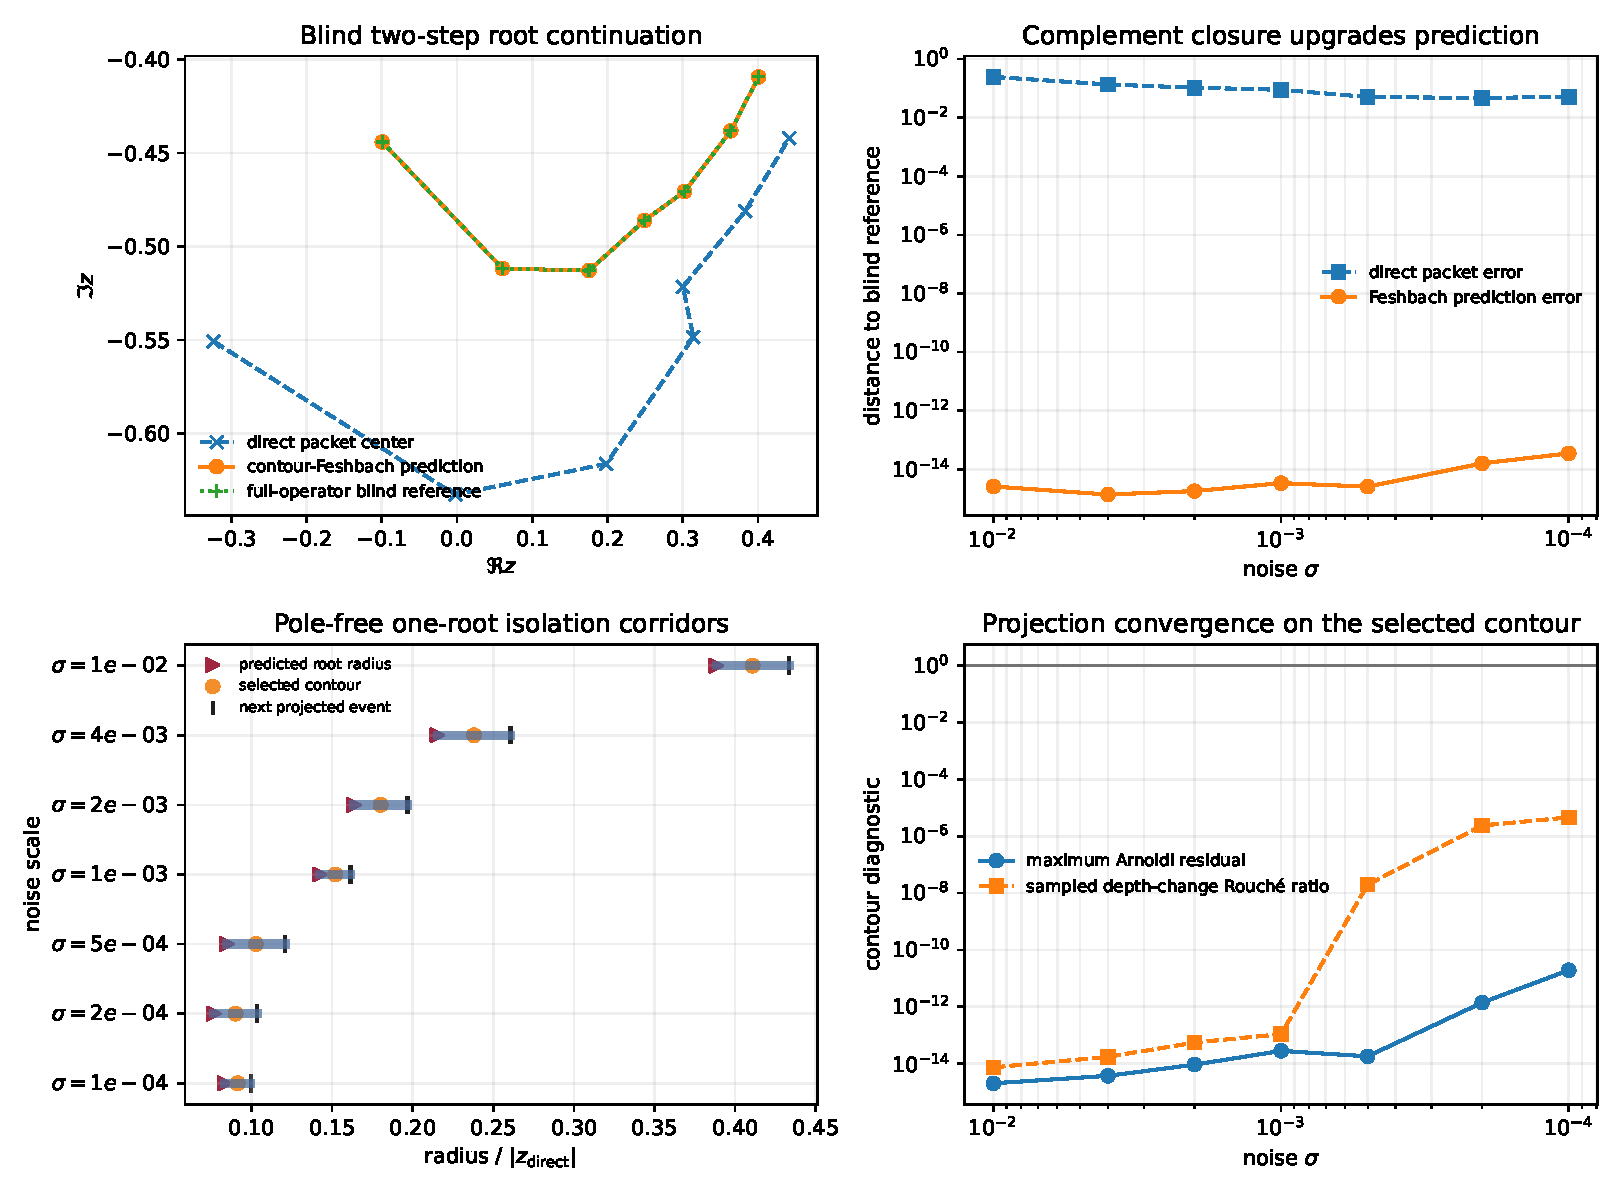
\includegraphics[width=\textwidth]{figures/contour_feshbach_summary.pdf}
\caption{Baseline root prediction and contour diagnostics.  Top left: the
direct packet centers miss the reference track, while the contour-Feshbach
roots lie on it.  Top right: direct and Feshbach errors.  Bottom left:
normalized one-root corridors, with the final contour at each midpoint.
Bottom right: floating Arnoldi residual bounds and sampled depth-change
Rouch\'e ratios.}
\label{fig:summary}
\end{figure}

\subsection{A renormalized contour, not a fixed circle}

The target-root radius relative to $|z_{\rm d}|$ changes from $0.3884$ at
$\sigma=10^{-2}$ to $0.0834$ at $10^{-4}$.  The selected contour factor
therefore changes from $0.4110$ to $0.0915$.  A fixed relative circle would
either miss the target at coarse noise or cross projected pole--zero
clusters at fine noise.  The computed route is explicitly nonuniform: the
contour must be centered and rescaled at each noise level.

The absolute corridor widths lie between $0.0101$ and $0.0288$; the relative
widths lie between $0.0161$ and $0.0454$.  They are not monotone, so no
power-law extrapolation is fitted.  The important finite-range fact is that
all seven corridors remain open, while the smallest one is narrow enough
that coarse contour placement would be unsafe.

\begin{figure}[H]
\centering
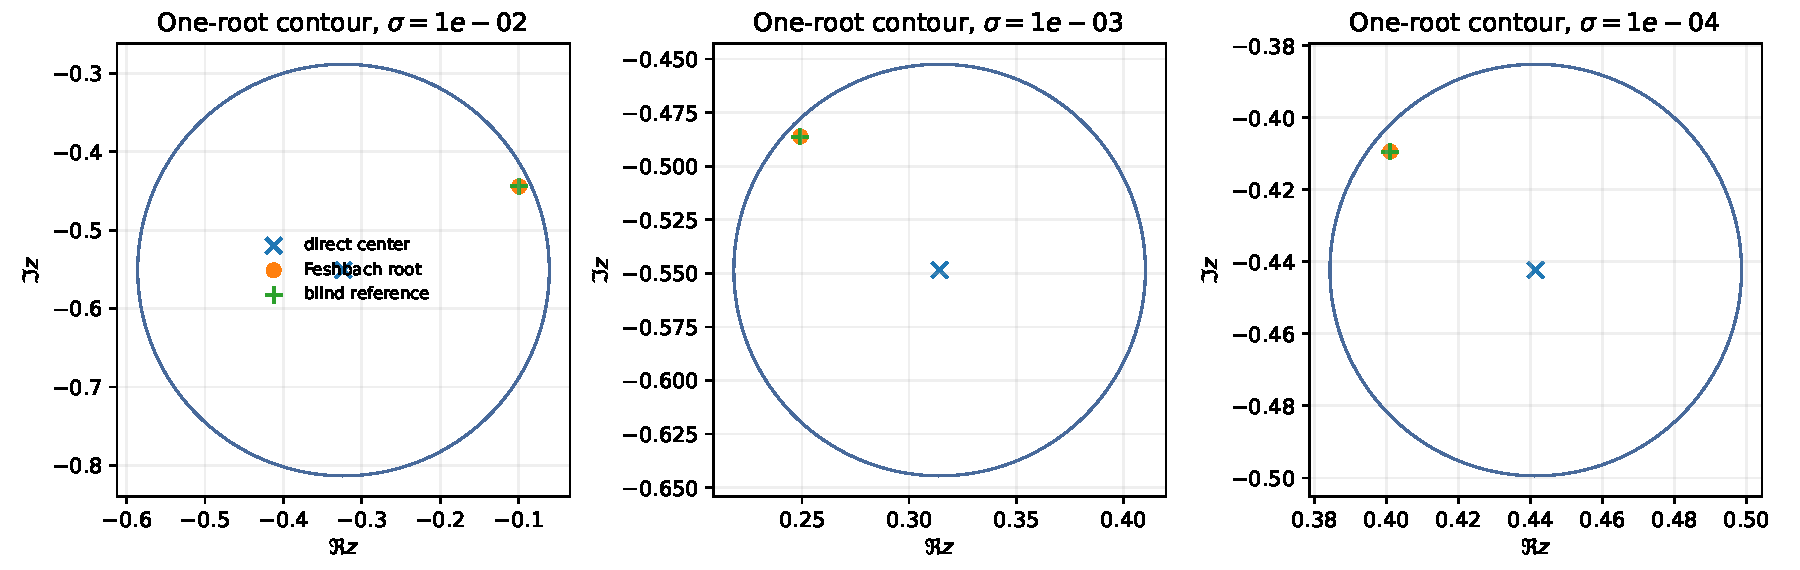
\includegraphics[width=\textwidth]{figures/selected_one_root_contours.pdf}
\caption{Representative optimized circles.  The center is selected from the
direct packet matrix; the contour-Feshbach root is computed before the
full-matrix reference is revealed.  The target and reference markers overlap
at plotting resolution.}
\label{fig:selected-contours}
\end{figure}

\subsection{Depth and contour-node convergence}

At depth $J-8$, the root changes from its depth-$J$ value by at most
$5.18\times10^{-9}$; at depth $J$ the residual bound is at most
$1.93\times10^{-11}$.  The two quantities need not have the same scale in a
nonnormal problem.  The sampled matrix-Rouch\'e ratio between $J-8$ and $J$,
evaluated on 128 contour nodes, is below one at all scales and at most
$4.59\times10^{-6}$.  This strongly
supports projected depth stability but remains subject to the qualification
after \cref{eq:sampled-rouche}.

\begin{figure}[H]
\centering
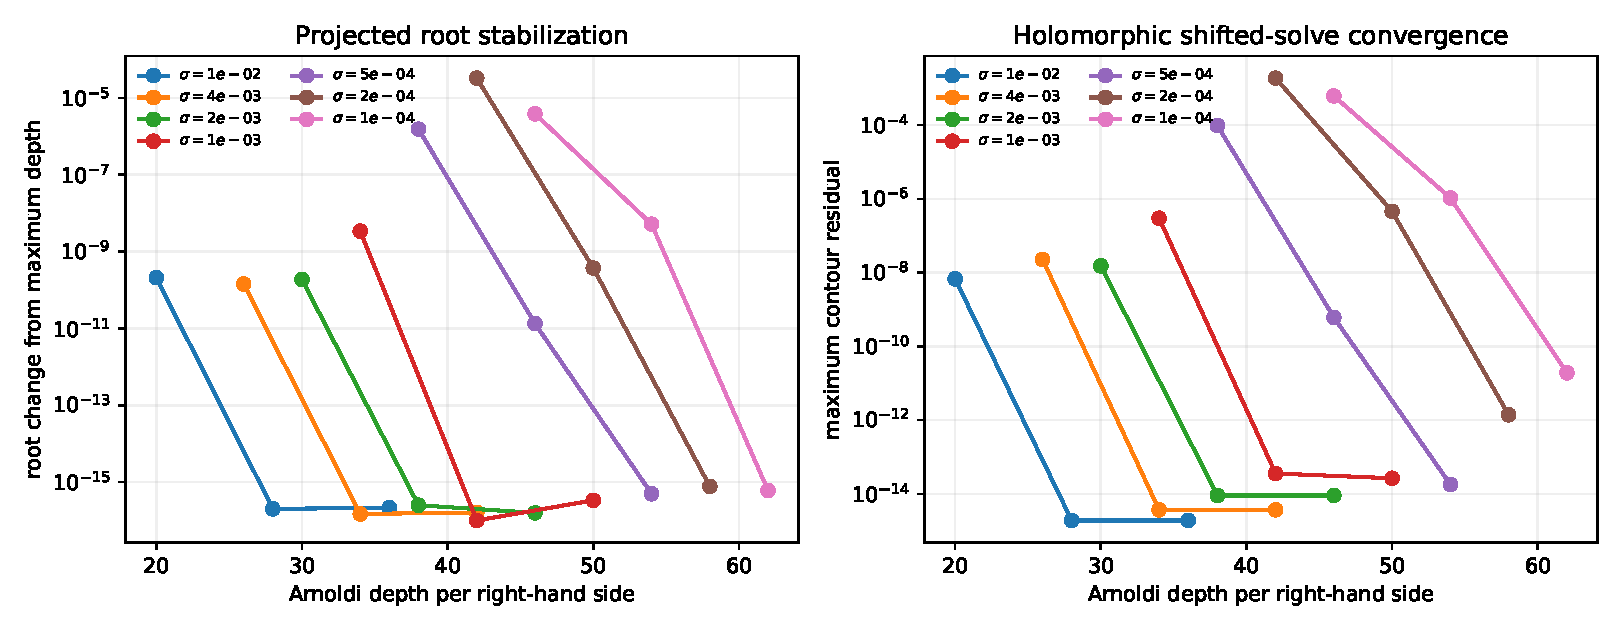
\includegraphics[width=\textwidth]{figures/arnoldi_depth_convergence.pdf}
\caption{Convergence with the number of Arnoldi vectors per right-hand side.
At the smallest scales, shallow spaces visibly miss the converged root, but
the prescribed maximum depths reach the floating recurrence floor.}
\label{fig:depth}
\end{figure}

All node counts from 64 through 512 return integer winding one on every
optimized contour.  At 512 nodes the maximum determinant phase increment is
$0.273<\pi$, the largest Cauchy count error is
$1.01\times10^{-12}$, and the largest Cauchy-centroid error against the
Newton root is $4.27\times10^{-14}$.

\begin{figure}[H]
\centering
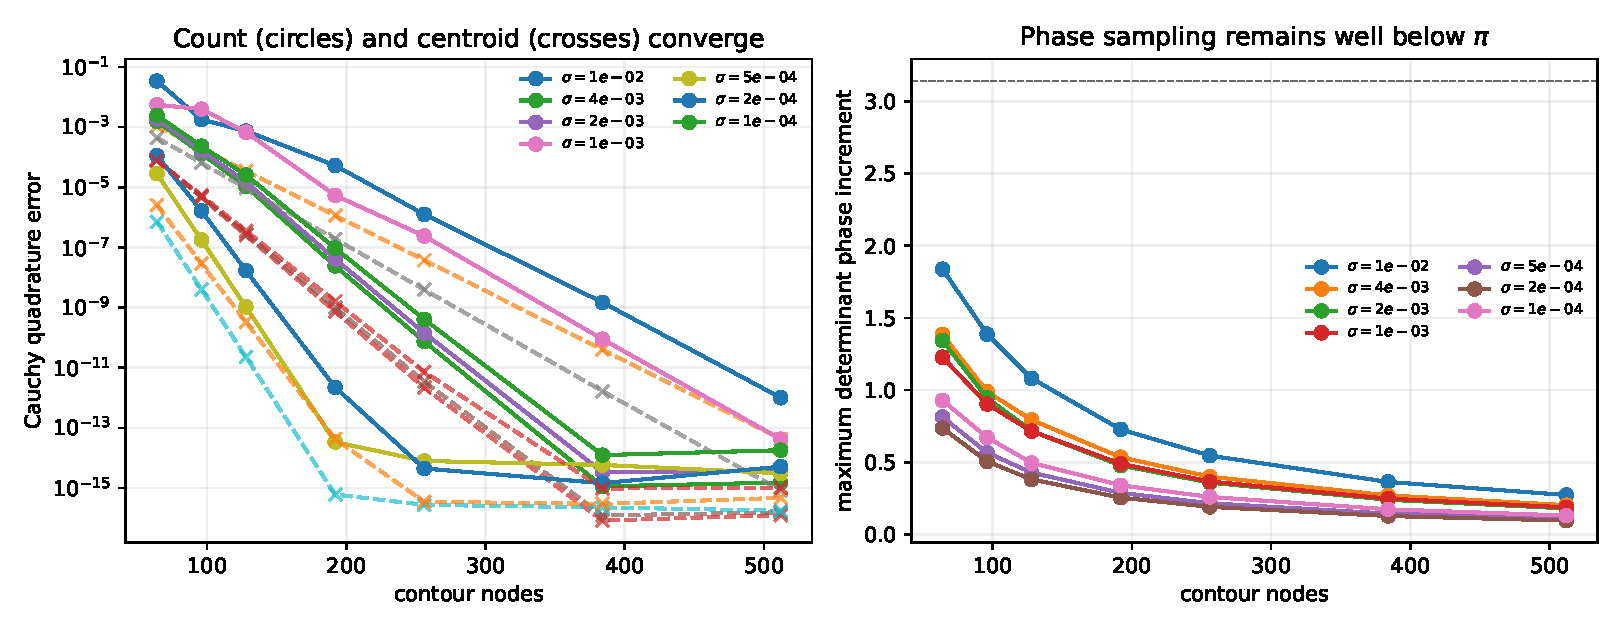
\includegraphics[width=\textwidth]{figures/contour_node_stability.pdf}
\caption{Contour quadrature refinement.  The Cauchy count and first-moment
centroid converge rapidly, while adjacent determinant phases remain safely
below the phase-aliasing threshold $\pi$.}
\label{fig:nodes}
\end{figure}

\section{Packet-window robustness}
\label{sec:window}

The packet half-width is a modeling choice, so reproducing one root only at
the baseline value six would be insufficient.  We rebuild the complete
Feshbach model at widths five and seven for $\sigma=10^{-3}$ and $10^{-4}$.
The direct center, complement, Arnoldi bases, projected poles, discovery
scan, and optimized contour all change with the window.  The frozen
full-matrix reference is used only after each root is selected.

\begin{table}[H]
\centering
\caption{Packet-window audit.  Every row has winding/poles/zeros $=1/0/1$.}
\label{tab:window}
\resizebox{\textwidth}{!}{%
\begin{tabular}{rrrrrrr}
\toprule
$\sigma$ & window & $\operatorname{cond}(\text{Gram})$ & direct error & Feshbach error & residual bound & corridor width\\
\midrule
$10^{-3}$ & 5 & 1.2722 & $8.990\times10^{-2}$ & $3.24\times10^{-15}$ & $2.76\times10^{-14}$ & $1.200\times10^{-2}$\\
$10^{-3}$ & 6 & 1.2725 & $9.005\times10^{-2}$ & $3.24\times10^{-15}$ & $2.81\times10^{-14}$ & $1.200\times10^{-2}$\\
$10^{-3}$ & 7 & 1.2725 & $9.005\times10^{-2}$ & $2.73\times10^{-15}$ & $2.99\times10^{-14}$ & $1.200\times10^{-2}$\\
$10^{-4}$ & 5 & 1.1148 & $4.801\times10^{-2}$ & $6.01\times10^{-13}$ & $3.14\times10^{-10}$ & $9.900\times10^{-3}$\\
$10^{-4}$ & 6 & 1.1196 & $5.213\times10^{-2}$ & $3.45\times10^{-14}$ & $1.93\times10^{-11}$ & $1.005\times10^{-2}$\\
$10^{-4}$ & 7 & 1.1198 & $5.228\times10^{-2}$ & $1.76\times10^{-14}$ & $9.56\times10^{-12}$ & $1.005\times10^{-2}$\\
\bottomrule
\end{tabular}}
\end{table}

The smallest-window, smallest-noise case is the least accurate, as its
residual bound and root error both increase.  They remain small compared
with the direct error, and the pole-free corridor stays open.  Hence the
single-root result is stable under this finite packet-window variation, not
exactly invariant under arbitrary packet choices.

\begin{figure}[H]
\centering
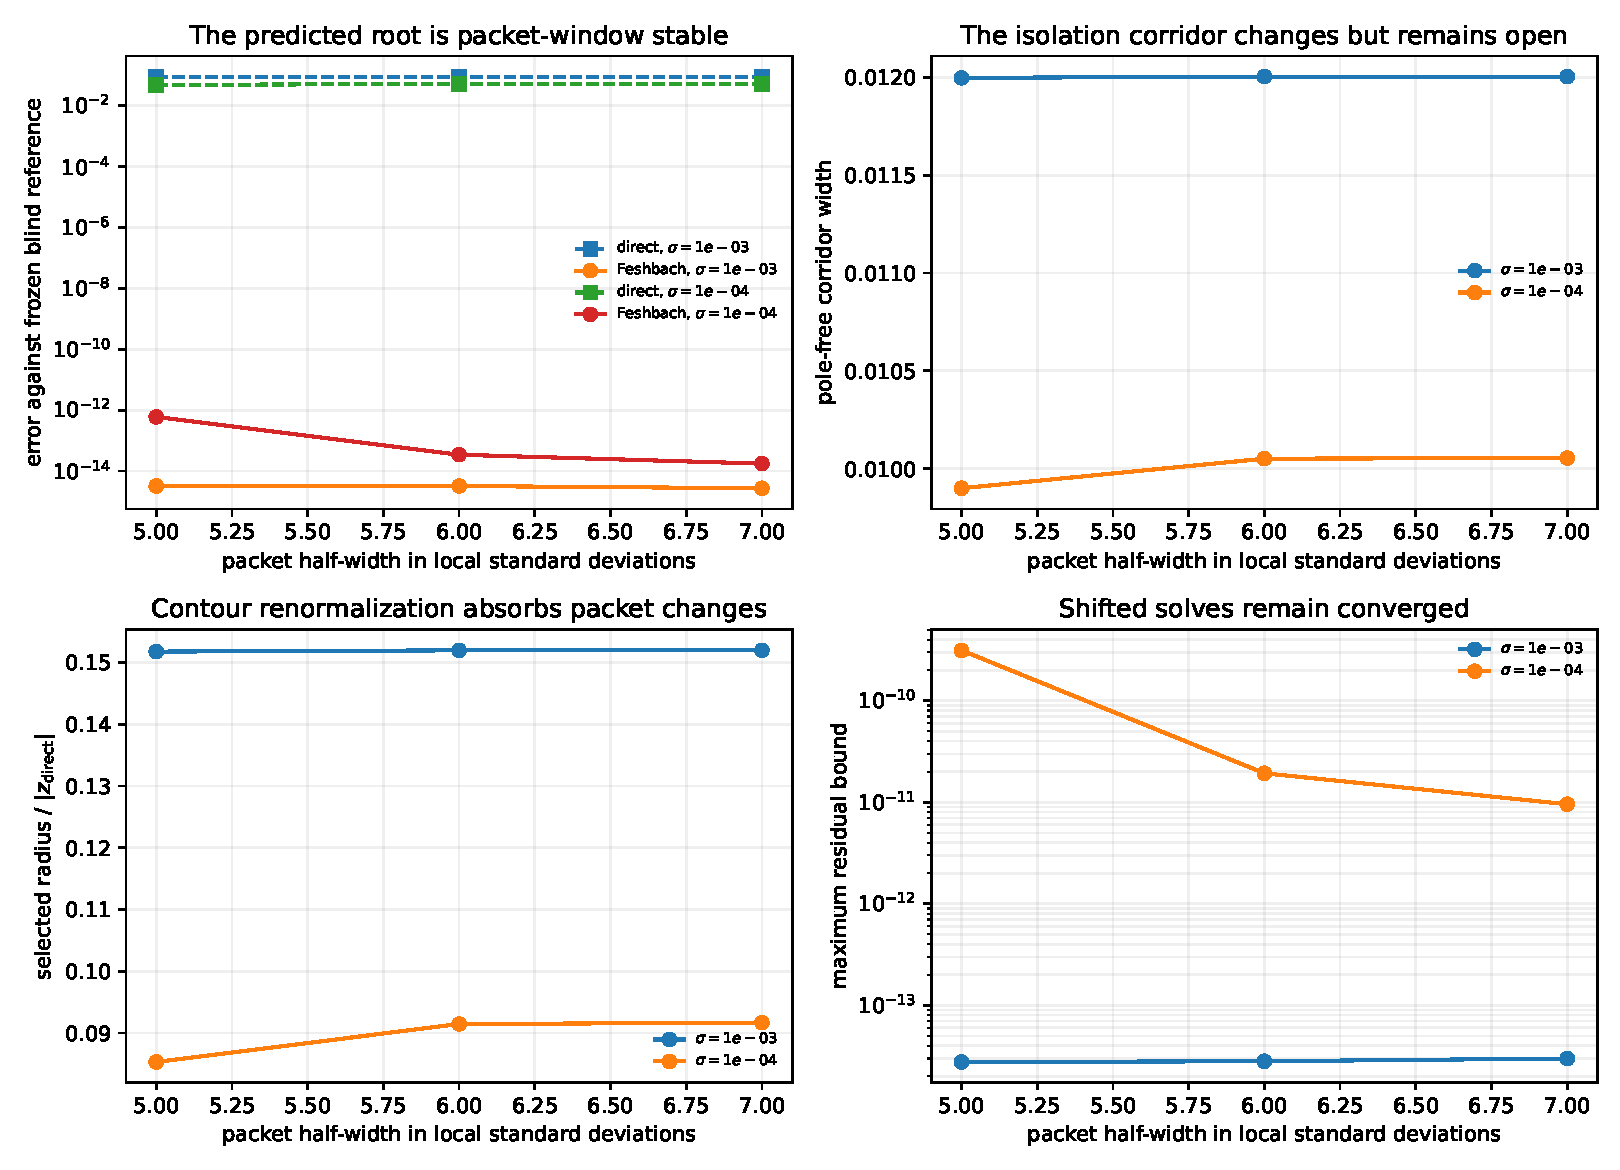
\includegraphics[width=\textwidth]{figures/packet_window_root_stability.pdf}
\caption{Packet-window robustness at two representative scales.  The direct
matrix and selected contour move with the packet, but the predicted physical
root remains stable.}
\label{fig:window}
\end{figure}

\section{What is established and what remains open}
\label{sec:limits}

The computation changes the status of the packet-complement route, but only
within a clearly delimited hierarchy.

\subsection{Exact finite-dimensional conclusions}

The following statements require no numerical hypothesis beyond the stated
invertibility conditions.

\begin{itemize}
 \item The oblique packet decomposition gives the exact determinant and
 compressed-resolvent identities in \cref{thm:exact-feshbach}.
 \item The Feshbach winding is the full-minus-external eigenvalue count in
 \cref{thm:argument-principle}.
 \item The shifted Arnoldi model is one rational, meromorphic matrix
 function, not unrelated pointwise fits.
 \item Its determinant is exactly the Schur complement of $M_J$, giving the
 zero-minus-pole identity in \cref{thm:projected-determinant}.
 \item The exact-model error obeys \cref{eq:feshbach-error-identity}, and
 \cref{eq:exact-rouche-condition} is sufficient to transfer the count.
\end{itemize}

\subsection{Finite floating-point evidence}

For the seven specified sparse matrices and six window variants, the
recorded data support all of the following.

\begin{itemize}
 \item A target-free packet center leads to a pole-free contour of projected
 winding one.
 \item Phase winding and augmented eigenvalue counting agree.
 \item The projected root stabilizes with Arnoldi depth and contour nodes.
 \item The prediction, frozen before the reference solve, matches the unique
 captured full-matrix eigenvalue in the contour.
 \item The required circle is nonuniform in $\sigma$ but an isolation
 corridor remains open throughout the computed range.
\end{itemize}

These are stronger than inserting a known eigenpair into an exact block
equation: the eigenvalue is now independently reconstructed from the
packet, complement action, and contour.  They are weaker than a validated
spectral theorem because every phase, residual, and reference eigenvalue is
still floating point.

\subsection{The next rigorous obstruction}

The principal missing estimate is not another root finder.  It is a uniform
or scale-renormalized upper bound for
\[
 \sup_{z\in\Gamma_\sigma}
 \|(z\Id-B_\sigma)^{-1}\|.
\]
RH-23 gave growing lower bounds, so a naive uniform-small-complement
argument is unavailable.  A useful upper bound must respect nonnormality and
the shrinking one-root corridor.  Possible routes include validated
pseudospectral enclosures, interval block solves on contour arcs, or a
Grushin formulation with explicit inverse estimates
\citep{TrefethenEmbree2005,SjoestrandZworski2007}.  Without such a bound,
small residuals and depth agreement cannot close
\cref{eq:scalar-rouche-bound} rigorously.

Three further issues remain.

\begin{enumerate}
 \item The independent column realizations duplicate external Ritz poles.
 A common block or rational Krylov realization could separate genuine
 external spectral events from near-cancelling realization clusters.
 \item The finite-section rule $n\sigma=20.48$ must be embedded in a
 discretization-convergence argument, followed by a controlled
 $\sigma\downarrow0$ limit.  The present seven points do not establish either
 limit.
 \item The contour follows one selected outer resonance.  Extending the
 construction to a multi-root region requires resolving adjacent physical
 roots and external poles without losing phase or conditioning control.
\end{enumerate}

\section{Conclusion}
\label{sec:conclusion}

The packet-complement construction has advanced from a closure identity for
an already known eigenmode to an independent finite-matrix spectral
prediction.  Exact Feshbach algebra turns the desired eigenvalue count into
a determinant winding.  Shift-invariant Arnoldi reduction preserves the
analytic spectral parameter, and an augmented realization makes every
projected zero-minus-pole count independently checkable.  On seven physical
discretizations, the resulting contour has one root and no projected pole,
and its root agrees with a later full-matrix reference to between
$10^{-15}$ and $10^{-14}$ in the baseline.  The result survives packet-window
variation, Arnoldi-depth variation, and contour refinement.

The positive conclusion is therefore specific: a renormalized nonuniform
Feshbach route is numerically viable and can predict the selected physical
resonance.  The equally important limitation is specific: a validated upper
bound on the exact external resolvent is still absent.  That bound, rather
than further pointwise agreement, is the next mathematical gate.

\appendix

\section{Reproducibility and stored artifacts}
\label{app:reproducibility}

The repository directory contains:

\begin{itemize}
 \item the generic package \texttt{src/contour\_feshbach}, implementing
 column-wise Arnoldi models, projected determinants, Cauchy counts, Newton
 refinement, and sampled Rouch\'e comparisons;
 \item six unit tests for Arnoldi residuals, analytic derivatives, augmented
 determinant factorization, zero-minus-pole winding, Newton refinement, and
 sampled matrix-Rouch\'e diagnostics;
 \item \texttt{experiments/run\_contour\_feshbach\_audit.py}, which performs
 the blind seven-scale calculation;
 \item \texttt{experiments/run\_packet\_window\_audit.py}, which performs the
 two-scale window variation;
 \item committed CSV, JSON, small serialized rational models, and all plotted
 figures.
\end{itemize}

The baseline is reproduced with
\begin{verbatim}
PYTHONPATH=src OPENBLAS_NUM_THREADS=16 /root/math/.venv/bin/python \
  experiments/run_contour_feshbach_audit.py
\end{verbatim}
and the window audit with
\begin{verbatim}
PYTHONPATH=src:experiments OPENBLAS_NUM_THREADS=16 \
  /root/math/.venv/bin/python experiments/run_packet_window_audit.py
\end{verbatim}
Figures can be regenerated from committed tabular data using \texttt{--reuse}.
SHA-256 hashes of the experiment and algebra sources are recorded in the
summary JSON files.  The seven baseline rational models occupy less than one
megabyte in compressed form, so contour and depth checks can be repeated
without rebuilding the large sparse operators.

\bibliographystyle{plainnat}
\bibliography{references}

\end{document}
